\documentclass[fr,license=none]{../../../eplexercises}

\usepackage{enumitem} % Enumeration avec des lettres
\usepackage{listings} % Code

\DeclareMathSizes{11}{19}{13}{9}   %  Pour un texte de taille 11
\newcommand{\reels}{\mathbb{R}}
\newcommand{\naturels}{\mathbb{N}}
\newcommand{\nieme}{$\mathrm{n^{i\`eme} }$}

\hypertitle{Méthodes de conception de programmes}{6}{INGI}{1122}
{Florian Thuin\and Eddy Ndizera}
{José Vander Meulen}

\section*{Principe de récurrence} 
  \[
    (P\langle0\rangle \textrm{ et } P\langle n\rangle \Rightarrow P\langle n+1\rangle) \Rightarrow (P\langle n\rangle \forall n)
  \]


\section*{Principe d'induction complète}
  \[
    ((P\langle0\rangle \textrm{ et } P\langle1\rangle \textrm{ et } ... \textrm{ et } P\langle n-1\rangle) \Rightarrow P\langle n\rangle) \Rightarrow (P\langle n\rangle \forall n) 
  \]


  	
\section*{Exercice 1.1.1.1.1}
      
      \paragraph{Prouvez par récurrence}
      
      \begin{center}
       \begin{tabular}{ll}
	  $\sum_{i=0}^{n} i^{2} = \frac{n*(n+1)*(2n+1)}{6}$ & $\forall n \in \mathbb{N}$
       \end{tabular}
      \end{center}
      
      \paragraph{$\mathbf{P\langle 0\rangle}$}
      
      \[
       \sum_{i=0}^{0} i^{2} = 0^{2} = 0 = \frac{0*(0+1)*(2*0+1)}{6}
      \]
      
      \paragraph{Hypothèse} $P\langle n\rangle \Rightarrow P\langle n+1\rangle$
      
      \[
       \sum_{i=0}^{n+1} i^{2} = \big(\sum_{i=0}^{n} i^{2}\big) + (n+1)^{2}
      \]
      
      \[
       = \frac{n*(n+1)*(2n+1)}{6} + \frac{6*(n+1)^{2}}{6}
      \]
      
      \[
       = \frac{(n+1)* \big(n*(2n+1)\big)}{6} + \frac{(n+1)*\big(6*(n+1)\big)}{6}
      \]
      
      \[
       = \frac{(n+1)* \big(n*(2n+1) + 6*(n+1)\big)}{6}
      \]
      
      \[
       = \frac{(n+1)* \big(2n^{2}+ 7n + 6\big)}{6}
      \]
      
      \[
       = \frac{(n+1)* \big((n+2)*(2n+3)\big)}{6}
      \]
      
      \[
       = \frac{(n+1)* \Big(\big((n+1)+1\big)*\big(2(n+1)+1\big)\Big)}{6}
      \]
      
\section*{Exercice 1.1.1.1.2}
      
      \paragraph{Prouvez par récurrence}
      
      \begin{center}
       \begin{tabular}{ll}
	  $\sum_{i=0}^{n} i^{3} = \frac{n^{2}(n+1)^{2}}{4}$ & $\forall n \in \mathbb{N}$
       \end{tabular}
      \end{center}
      
      \paragraph{$\mathbf{P\langle 0\rangle}$}
      
      \[
       \sum_{i=0}^{0} i^{3} = 0^{2} = 0 = \frac{0*(0+1)^{2}}{4}
      \]
      
      \paragraph{Hypothèse} $P\langle n\rangle \Rightarrow P\langle n+1\rangle$
      
      \[
       \sum_{i=0}^{n+1} i^{3} = \big(\sum_{i=0}^{n} i^{3} \big) + (n+1)^{3}
      \]
      \[
       = \frac{n^{2}(n+1)^{2}}{4} + (n+1)^{3}
      \]
      \[
       = \frac{n^{2}(n+1)^{2}}{4} + \frac{4(n+1)^{3}}{4}
      \]
      \[
       = \frac{(n+1)^{2}(n^{2}+4(n+1))}{4}
      \]
      \[
       = \frac{(n+1)^{2}(n^{2}+4n+4)}{4}
      \]
      \[
       = \frac{(n+1)^{2}(n+2)^{2}}{4}
      \]


\section*{Exercice 1.1.1.1.3}
      
	  \paragraph{Prouvez par récurrence}      
      
      \begin{center}
       \begin{tabular}{ll}
	  $\sum_{i=0}^{n} x^{i} = \frac{x^{n+1}-1}{x-1}$ & $\forall n \in \mathbb{N}$ et $x \neq -1$ 
       \end{tabular}
      \end{center}
      
	  \paragraph{$\mathbf{P\langle 0\rangle}$}
	      
	  \[
       \sum_{i=0}^{0} x^{i} = x^{0} = 1 = \frac{x - 1}{x - 1}
      \]
      
      
	  \paragraph{Hypothèse} $P\langle n\rangle \Rightarrow P\langle n+1\rangle$
	  
	  \[
	  	\sum_{i=0}^{n+1} x^{i} = \big(\sum_{i=0}^{n} x^{i} \big) + x^{n+1}
	  \]
	  \[
	  	= \frac{x^{n+1} - 1}{x - 1} + x^{n+1}
	  \]
	  \[
	  	= \frac{x^{n+1} - 1 + x^{n+1} (x - 1)}{x - 1}
	  \]
	  \[
	  	= \frac{x^{n+1} - 1 + x^{n+2} - x^{n+1}}{x - 1}
	  \]
	  \[
	  	= \frac{x^{n+2} - 1}{x - 1}
	  \]
	  \[
	  	= \frac{x^{(n+1)+1} - 1}{x - 1}
	  \]
	        

\section*{Exercice 1.1.1.1.4}
      
	  \paragraph{Prouvez par récurrence}      
      
      \begin{center}
       \begin{tabular}{ll}
	  $\sum_{i=0}^{n} 2^{i} = 2^{n+1} - 1$ & $\forall n \in \mathbb{N}$ 
       \end{tabular}
      \end{center}
      
	  \paragraph{$\mathbf{P\langle 0\rangle}$}    
	  
	  \[
	  	\sum_{i=0}^{0} 2^{i} = 2^{0} = 1 = 2^{1} - 1
	  \]  
	  
	  \paragraph{Hypothèse} $P\langle n\rangle \Rightarrow P\langle n+1\rangle$
	  
	  \[
	  	\sum_{i=0}^{n+1} 2^{i} = \big(\sum_{i=0}^{n} 2^{i} \big) + 2^{n+1}
	  \]
	  \[
	  	= 2^{n+1} - 1 + 2^{n+1}
	  \]
	  \[
	  	= 2.2^{n+1} - 1
	  \]
	  \[
	  	= 2^{(n+1)+1} - 1
	  \]
	  
	  
\section*{Exercice 1.1.1.1.5}
      
	  \paragraph{Prouvez par récurrence}      
      
      \begin{center}
       \begin{tabular}{ll}
	  $(1 + p)^{n} \geq 1 + np$ & $\forall n \in \mathbb{N}$ et $p > -1$
       \end{tabular}
      \end{center}
      
	  \paragraph{$\mathbf{P\langle 0\rangle}$} 
	  
	  \[
	  	(1 + p)^{0} = 1 \geq 1 = 1 + 0.p
	  \]
	  
	  \paragraph{Hypothèse} $P\langle n\rangle \Rightarrow P\langle n+1\rangle$
	  
	  \[
	  	(1 + p)^{n+1} = (1 + p)(1 + p)^{n}
	  \]
	  \[
	  	\geq (1 + p)(1 + np)
	  \]
	  (Hypothèse de récurrence et parce que $p > -1 \Rightarrow 1 + p > 0$)
	  \[
	  	= 1 + (n + 1)p + np^{2}
	  \]
	  \[
	  	\geq 1 + (n + 1)p
	  \]
	  (parce que $np^{2} \geq 0$ car $n \geq 0$ et $p^{2} \geq 0$)
 
\section*{Exercice 1.1.1.2}
      
      \[
       F_{0} = 0
      \]
      \[
       F_{1} = 1
      \]
      
      \begin{center}
	\begin{tabular}{ll}
	  $F_{i+2} = F_{i+1} + F_{i}$ & $\forall \in \mathbb{N}$
	\end{tabular}
      \end{center}
      
      \paragraph{Prouvez}
      
      \begin{center}
	\begin{tabular}{ll}
	$F_{n+1} F_{n-1} - F_{n}^2 = (-1)^{n}$ & $\forall n \in \mathbb{N} \setminus \{0\} $
	\end{tabular}
      \end{center}
      
      \[
       (F_{n} + F_{n-1}) (F_{n-2} + F_{n-3}) - F_{n}^{2} = (-1)^{n}
      \]
      
      \paragraph{P<1>}
      
      \[
       F_{2} F_{0} - F_{1}^{2} = (0+1)*0 - 1^{2} = -1 = -1^{1}
      \]
      
      \paragraph{Hypothèse} $P\langle n\rangle \Rightarrow P\langle n+1\rangle$
      
      \[
       F_{n+2} F_{n} - F_{n+1}^{2}
      \]
      
      \[
       = (F_{n+1} + F_{n}) * F_{n} - F_{n+1} F_{n+1}
      \]
      
      \[
       = F_{n} F_{n+1} + F_{n}^{2} - (F_{n} + F_{n+1}) F_{n+1}
      \]
      
      \[
       = F_{n} F_{n+1} + F_{n}^{2} - F_{n} F_{n+1} - F_{n-1} F_{n+1}
      \]
      \[
       = - (F_{n-1} F_{n+1} - F_{n}^{2})
      \]
      \[
       = - ((-1)^{n})
      \]
      \[
       = (-1)^{n+1}
      \]
      
\section*{Exercice 1.2.1.1}

\nosolution

\section*{Exercice 1.2.1.2}
      
      Un ensemble $E$ de taille $n$ : $C_{n}^{m}$ (sans utiliser $C_{n}^{m} = \frac{n!}{m!(n-m)!}$)
      
      \begin{enumerate}[label=(\alph*)]
       \item \begin{tabular}{p{3.5cm}l} $C_{n}^{0} = C_{n}^{n} = 1$ & $\forall n \in \mathbb{N}$ \end{tabular}
       \item \begin{tabular}{p{3.5cm}l} $C_{n}^{m} = 0$ & si $m > n$ \end{tabular}
       \item \begin{tabular}{p{3.5cm}l} $C_{n}^{m} = C_{n-1}^{m} + C_{n-1}^{m-1} $ & si $m,n \geq 1$ \end{tabular}
      \end{enumerate} \bigskip
      
      \begin{enumerate}[label=(\alph*)]
       \item \begin{itemize}
              \item Il n'existe qu'un seul sous-ensemble de $E$ de taille $0$ : l'ensemble vide. Donc, $C_{n}^{0} = 1$.
              \item Il n'existe qu'un seul sous-ensemble de $E$ de taill $n$ : l'ensemble $E$ lui-même. Donc $C_{n}^{n} =1$
             \end{itemize}
      \item \begin{itemize}
             \item Il n'existe pas de sous-ensemble de $E$ contenant plus d'éléments que $E$. Donc $C_{n}^{m} = 0$ si $ m>n$
            \end{itemize}
      \item Soit un élément $e$ de $E$ (il existe car $n \geq 1$). On peut partitionner l'ensemble des sous-ensembles de taille $m \geq 1$ de l'ensemble $E$ (de taille $n \geq 1$) en deux :
      
      \begin{itemize}
       \item les sous-ensembles contenant $e$, il y en a autant que de sous-ensembles de taille $n-1$ de l'ensemble $E \setminus \{e\}$ c-à-d $C_{n-1}^{m-1}$ sous-ensembles.
       \item les sous-ensembles ne contenant pas $e$, il y en a autant que de sous-ensembles de taille $m$ de l'ensemble $E \setminus \{e\}$ c-à-d $C_{n-1}^{m}$ sous-ensembles puisqu'il s'agit d'une partition $C_{n}^{m} = C_{n-1}^{m-1} + C_{n-1}^{m} $.
      \end{itemize}

      \end{enumerate}
      
\section*{Exercice 1.2.1.3}
      
      \begin{enumerate}
       \item \begin{tabular}{p{3cm}l} $T_{n+1} + T_{n} = 2^{n+2}$ & $\forall n \in \mathbb{N}$ \end{tabular}
       \item \begin{tabular}{p{3cm}l} $ T_{n} = \frac{2^{n+2} - 1}{3} $ & si $n$ est pair \end{tabular}
       \item \begin{tabular}{p{3cm}l} $ T_{n} = \frac{2^{n+2} + 1}{3} $ & si $n$ est impair \end{tabular}
      \end{enumerate} \bigskip
      
      \[
       p_{0} \Rightarrow p_{1}
      \]
      \[
       (p_{0} \Rightarrow p_{1}) \Rightarrow p_{2}
      \]
      \[
       T_{n} = ((...((p_{0} \Rightarrow p_{1}) \Rightarrow p_{2}) ... ) \Rightarrow p_{n})
      \]
      
      Nous avons $n+2$ variables $p_{0},p_{1},...,p_{n},p_{n+1}$
      
      $F\langle n\rangle \equiv ((...((p_{0} \Rightarrow p_{1}) \Rightarrow p_{2}) ... ) \Rightarrow p_{n})$
      
      $F\langle n+1\rangle \equiv F\langle n\rangle \Rightarrow p_{n+1}$
      
      $T_{n}$ est l'interprétation de ce qui rend vrai $F\langle n\rangle$
      
      \begin{multicols}{2}
      
      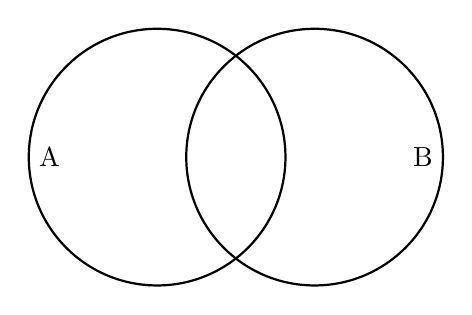
\begin{tikzpicture}
	\tikzstyle{ensemble}=[draw, circle, thick, text width=3cm]
	
	\node[ensemble] (A) at (0,0) {A};
	\node[ensemble, align=right] (B) at (2,0) {B};
      \end{tikzpicture}
     
      \columnbreak
      
      \noindent $A = \{ f \in I \mid f \models F\langle n+1\rangle \} $
      
      \noindent $B = \{ f \in I \mid f \nvDash F\langle n+1\rangle \} $
      
      \noindent $\#I = \#A + \#B$
      
     \end{multicols}
     
     $\#A = T_{n+1}$
     
     $\#B = T_{n}$
     
     $F\langle n+1\rangle \} : \underbrace{(F\langle n\rangle}_{V} \Rightarrow \underbrace{p_{n+1}}_{F})$
     
     $T_{n+1} + T_{n} = \#A + \#B = \#I = \overbrace{2^{n+2}}^{n+2 \textrm{ variables}}$
     
     \bigskip
     \begin{tabular}{ll}
     $P\langle n\rangle$ : & si $n$ est pair alors $T_{n} = \frac{2^{n+2} -1}{3}$ \\
     & si $n$ est impair alors $T_{n} = \frac{2^{n+2} +1}{3}$
     \end{tabular}
     \bigskip
     
     \begin{tabular}{lp{4cm}l}
     $p\langle0\rangle :$ & $T_{0} = \frac{2^{2}-1}{3}$ & $F\langle0\rangle : p_{0}$ \\
     & $T_{0} = 1 \frac{4-1}{3} = \frac{2^{2}-1}{3}$ & $P_{0} \Rightarrow V $ ; $P_{0} \Rightarrow F$\\
     \end{tabular}
     \bigskip
     
     $\mathbf{P\langle n+1\rangle}$
     
     \begin{multicols}{2}
     n est pair
     
     $P\langle n \rangle \Rightarrow P\langle n+1\rangle$
     
     $T_{n+1} = 2^{n+2} - T_{n}$
     
     $ = 2^{n+2} - (\frac{2^{n+2}-1}{3}) $
     
     $ = \frac{3*2^{n+2} - 2^{n+2} +1}{3}$
     
     $ = \frac{2 * 2^{n+2} + 1}{3} = \frac{2^{n+3} +1 }{3}$
     
     \columnbreak
     n est impair
     
     raisonnement similaire que n est pair
     \end{multicols}
     
	\textbf{En utilisant le principe de récurrence:}  
	\begin{tabular}{p{3cm}l} $T_{n+1} + T_{n} = 2^{n+2}$ & $\forall n \in \mathbb{N}$ \end{tabular}. \\
	-Pour \textbf{n = 0} : \\
	$T_{1} + T_{0} = 3 + 1 = 4 = 2^{2}$\\
	En effet, si on se base sur les tables de vérités, on a bien que $T_{0} = 1$ et $T_{1} = 3$.
	\begin{center}
	
	
	\begin{tabular}{|c|}
  		\hline
  		 $p_{0}$ \\
  		\hline
  		V \\
  		F \\
  		\hline
	\end{tabular}
	\begin{tabular}{|c|c|c|}
  		\hline
  		 $p_{0}$ & $p_{1}$ & $p_{0} \Rightarrow p_{1}$ \\
  		\hline
  		V & V & V\\
  		V & F & F\\
  		F & V & V\\
  		F & F & V\\
  		\hline
	\end{tabular}
	\end{center} 
	
	-Pour \textbf{n+1} (en supposant que la propriété est vrai pour n):\\
	\[
		T_{n+2} + T_{n+1} = (2^{n+3} - T_{n+1}) + T_{n+1} = 2^{n+3}
	\]
	On a que $T_{n+2} = T_{n+1} + 2(2^{n+2} - T_{n+1}) = T_{n+1} + 2^{n+3} - 2T_{n+1}$. \\
	En effet $T_{n+1}$ correspond aux implications vraies jusqu'à $p_{n+1}$. Il suffit dès lors d'ajouter une implication avec $p_{n+2}$ vraie pour que les implications restent vraies.\\
	$(2^{n+2} - T_{n+1})$ correspond à toutes les implcations fausses jusqu'à $p_{n+1}$ et à qui il suffit d'ajouter un $p_{n+2}$ quelconque (vrai ou faux) pour que les implications deviennent vraies d'où $2(2^{n+2} - 2T_{n+1})$ possibilités. 
	$2^{n+2}$ est le nombre d'implications possibles jusqu'à $p_{n+1}$ et $T_{n+1}$ le nombre d'implications correctes. On en conclut que $(2^{n+2} - T_{n+1})$ est le nombre d'implications fausses. \\
	
	On vient de démontrer que la propriété est correcte par récurrence.
      
\section*{Exercice 1.2.1.4}

\nosolution

\section*{Exercice Syllabus Page 33 \no 2}
      
      On demande d'écrire une méthode d'en-tête
      
      static long bigC(int n, int m)
      
      pour calculer le nombre $C_{n}^{m}$ par la méthode du triangle de Pascal, c'est-à-dire en utilisant les formules de l'exercice 2 de la page 5. Attention, le but est d'obtenir un algorithme de complexité $O(mn)$. Bien sûr, l'algorithme ne peut pas faire de multiplications, seulement des additions.
      
      Les formules :
      
      $C_{n}^{0} = C_{n}^{n} = 1$ $\forall n \in \naturels $
      
      $C_{n}^{m} = 0$ si $n < m$
      
      $C_{n}^{m} = C_{n-1}^{m} + C_{n-1}^{m-1}$ si $m,n \ge 1$
      
      \subsection*{Découpe en sous-problèmes}
      
      \begin{enumerate}
       \item Construire la prochaine ligne du triangle de Pascal
       \item Construire la ligne qu'il nous faut
       \item Donner la valeur de $C_{n}^{m}$
      \end{enumerate}
      
      \paragraph{SP1} Construire la prochaine ligne
      
      \underline{En-tête} : public static long[] nextLine(long[] line)
      
      \underline{Pre} : line représente une ligne valide du triangle de Pascal ayant m+1 et m.
      
      \[
       1 \le m \le n
      \]
      
      \underline{Post} : les éléments de line restent inchangés tout au long du SP1
      
      \underline{Résultat} : la ligne suivante du triangle de Pascal
      
      \paragraph{SP2} Construire la ligne n
      
      \underline{En-tête} : public static long[] lastLine (int n, int m)
      
      \underline{Pré} : $1 \le m \le n$
      
      \underline{Post} : /
      
      \underline{Résultat} : La \nieme ligne du triangle de Pascal comprenant
      
      \[
       [C_{n}^{0}, C_{n}^{1}, C_{n}^{2}, ..., C_{n}^{m}]
      \]
      
      les éléments $C_{n}^{0},C_{n}^{1},...,C_{n}^{m}$
      
      \paragraph{PP} Calculer $C_{n}^{m}$
      
      public static long bigC(int n, int m)
      
      \underline{Pré} : $n, m \ge 0$
      
      \underline{Post} : -
      
      \underline{Résultat} : $C_{n}^{m}$
      
      \underline{Méthode} : 

      \begin{lstlisting}
	Si n < m alors 
	  return 0;
	Sinon /* m <= n */ :
	  Si m=0 || m=n alors
	    return 1;
	  sinon
	    long[] lastLine = lastLine(n, m);
	    return lastLine[m];
      \end{lstlisting}

      
\section*{TP 7 Exercice 1}
      
      Construire une variante de la recherche dichotomique, qui procède en deux étapes :
      
      \begin{enumerate}
       \item Déterminer l'indice i où la valeur cherchée peut se trouver
       \item Voir si l'élément y est
      \end{enumerate}
      
      \begin{center}
      \begin{tabular}{lccc}
      & & i & \\ \cline{2-4}
      $a$ : & \multicolumn{1}{|c|}{... < x} & \multicolumn{1}{c|}{} & \multicolumn{1}{c|}{x < ...} \\ \cline{2-4}
      \end{tabular}
      \end{center}
      
      S'il existe $i : 0 \le i < a.length$ tel que $a[i] = x$
      
      \subsection*{Découpe en sous-problèmes}
      
      \begin{enumerate}
       \item Trouver i
       \item Voir si x est présent
       \item PP
      \end{enumerate}
      
      \paragraph{SP1} Trouver i
      
      \underline{En-tête} : public static int trouverI(int[] a, int x)
      
      \underline{Pré} :
      \begin{itemize}
       \item a est trié en ordre croissant
       \item a est non null, a.length > 0
      \end{itemize}
      
      \underline{Post} : les éléments de a sont inchangés
      
      \underline{Résultat} : L'indice i tel que 
      
      \begin{itemize}
       \item -1 s'il n'existe pas d'indice i dans a tel que
	\subitem $\forall e : 0 \le e < i$ $a[e] < x$
	\subitem $\forall e : i < e' < a.length$ $a[e] > x$
       \item \underline{sinon} retourne i tel que
	\subitem $\forall e : 0 \le e < i$ $a[e] < x$
	\subitem $\forall e : i < e' < a.length$ $a[e] > x$
      \end{itemize}
      
      \paragraph{SP2} Si x est présent
      
      \underline{En-tête} : public static boolean isEqual(int[] a, int x, int i)
      
      \underline{Pré} :
      \begin{itemize}
       \item a est non null et a.length > 0 \&\&
       \item a est trié en ordre croissant \&\&
       \item $0 \le i < a.length$ \&\&
       \item $\forall e : 0 \le e < i$ $a[e] < x$ \& $\forall e' : i < e' < a.length$ $a[e'] > x$
      \end{itemize}
      
      \underline{Post} : les éléments de a restent inchangés
      
      \underline{Résultat} :
      \begin{itemize}
       \item true si $a[i]=x$
       \item false sinon
      \end{itemize}
      
      \paragraph{PP}
      
      \underline{En-tête} : public static boolean rd(int[] a, int x)
      
      \underline{Pré} : a non null et trié en ordre croissant
      
      \underline{Post} : les éléments de a restent inchangés
      
      \underline{Résultat} :
      \begin{itemize}
       \item true si x se trouvent dans le tableau a
       \item false sinon
      \end{itemize}
      
      \underline{Méthode}
      \begin{lstlisting}
	si a.length = 0 alors
	  return false;
	sinon /* a.length > 0 */
	  int i = trouverI(a, x);
	  si i < 0 alors return false
	  sinon return isEqual(a, x, i)
      \end{lstlisting}
      
      \underline{INV} :
      
      \begin{itemize}
       \item $0 \le i \le v < n = a.length$ \&\&
       \item $\forall j : 0 \le j < u$ : $a[j] < x$ (G) \&\&
       \item $\forall j : v < j < n$ : $a[j] > x$ (D)
      \end{itemize}
      
      \underline{INIT} :
      \begin{itemize}
       \item i = 0
       \item v = n - 1
      \end{itemize}
      
      \underline{H} : i = v
      
      \underline{ITER} :
      \begin{itemize}
       \item m := (i+v)/2
       \item si (a[m] < x) i:=m+1
       \item sinon si (a[m] > x) v:= m
      \end{itemize}
      
      \underline{CLOT} : return i
      
      \underline{Variant} : v-i
      
\section*{TP7 Exercice 2}
    
    La valeur la plus fréquente dans une vallée non stricte
    
    \[
     4,4,2,2,1,1,1,-5-5,0,0,0
    \]
    
    \[
     1,2,2,2,2,5,5,5
    \]
    
    v: la valeur la plus fréquente
    
    nV : le nombre de fois que la valeur apparaît
    
    \subsection*{Découpe en sous-problèmes}

      \begin{enumerate}
       \item Compter le nombre de valeurs successives égales à x, en partant de i comprises entre [i, j]
       \item Compter le nombre de valeurs successives égales à x, en partant de j, comprises entre [i,j]
       \item PP
      \end{enumerate}
      
      \paragraph{SP1}
      
      \underline{En-tête} : static int vpg(int[] a ,int x, int i, int j)
      
      \underline{Pré} : $0 \le i \le j < n$
      
      \underline{Post}  les éléments de a sont inchangés
      
      \underline{Résultat} : le ombre de valeurs successives égales à x à partir de a[i].
      
      \paragraph{PP}
      
      \underline{Pré} : a est non null et une vallée
      
      \underline{Post} : les éléemnts de a sont inchangés
      
      \underline{Résultat} : [v, nV]
      
      \underline{INV} :
      \begin{itemize}
       \item $0 \le i \le j < n$
       \item (v, nV) représente la valeur la plus fréquente dans les parties G et D de a, nV le nombre de fois que cette valeur apparaît.
      \end{itemize}
      
      \underline{INIT}
      \begin{itemize}
       \item j = n-1
       \item nV=0
       \item v=?
      \end{itemize}
      
      \underline{H} : i=j+1
      
      \underline{ITER}
      \begin{lstlisting}
	w = max(a[i], a[j])
	nW = 0
	i0 = vpg(a,w,i,j)
	nW := nW + i0
	i1 := i + i0
	j0 = vpd(a, w, i,j)
	nW = nW + I0
	j := j-j0
      \end{lstlisting}
      
      \begin{lstlisting}
      si nW > nV alors
	v = w
	nV = nW
      \end{lstlisting}
      
      \underline{CLOT} : return new int[] \{v, w\}

\end{document}
